\documentclass{ieeeaccess}
\usepackage{cite}
\usepackage{amsmath,amssymb,amsfonts}
\usepackage{algorithmic}
\usepackage{graphicx}
\usepackage{textcomp}
\usepackage{algorithm2e}
\usepackage{multirow}
\def\BibTeX{{\rm B\kern-.05em{\sc i\kern-.025em b}\kern-.08em
    T\kern-.1667em\lower.7ex\hbox{E}\kern-.125emX}}
\begin{document}
%\history{Date of publication xxxx 00, 0000, date of current version xxxx 00, 0000.}
\history{}
%\doi{10.1109/ACCESS.2017.DOI}
\doi{}

\title{Recent Research Progress on Cognition Capabilities of Service Robots}
\author{\uppercase{Hecheng Zhao}\authorrefmark{1},
\uppercase{Yuan Li\authorrefmark{2}, and Sukhan Lee}.\authorrefmark{3},
\IEEEmembership{Fellow, IEEE}}
\address[1]{Intelligent System Research Institute (ISRI),
Sungkyunkwan University, 16419, Suwon, South Korea (e-mail: hczhao@skku.edu)}
\address[2]{Benewake Co., Ltd., Beijing, China (ly@benewake.com)}
\address[3]{Intelligent System Research Institute (ISRI),
Sungkyunkwan University, 16419, Suwon, South Korea (e-mail:
lsh@ece.skku.ac.kr)}
%\tfootnote{This paragraph of the first footnote will contain support 
%information, including sponsor and financial support acknowledgment. For 
%example, ``This work was supported in part by the U.S. Department of 
%Commerce under Grant BS123456.''}

%\markboth
%{Author \headeretal: Preparation of Papers for IEEE TRANSACTIONS and JOURNALS}
%{Author \headeretal: Preparation of Papers for IEEE TRANSACTIONS and JOURNALS}

\corresp{Corresponding author: Sukhan Lee (e-mail: lsh@ece.skku.ac.kr).}

\begin{abstract}
This report summarizes the works which have been presented by the Intelligent Systems Research Institute of Sungkyunkwan University to the community of artificial intelligence and robotics. Five relevant articles published by the Institute during 2015 to 2018 are reviewed in order to exhibit the research progress made on cognitive capabilities of service robots. The Major Line Extraction algorithm has been proposed to exploit line features of the environments. This novel algorithm exhibits an improvement on extracting cursive lines with less discontinuities. Experimental results have shown that the algorithm outperforms a well-known method called the Line Segment Detector. Additionally, the Covariance Projection Filtering is a sensor filtering framework proposed for distributed sensory systems. The framework generalizes a filtering model for Gaussian linear systems. Comparing with Kalman filters, it provides an additional step for detecting data anomalies. For indoor environments, Wi-Fi fingerprints are of available landmarks for localizing robot positions. A new approach has been proposed based on the concept of "invariant received signal length statistics" that is able to overcome the instability of Wi-Fi signals. Experimental results show that this new method provides higher performance by 17\% in terms of success rate. For object detection, a new method has been proposed for detecting industrial objects with less textures. The method employees model-based point cloud matching within an adaptive Bayesian framework. Experiments show that such an approach achieves over 97.5\% of recognition rate. Later, a deep neural network has been integrated into such a framework. It adopts a Convolutional Neural Network based feature extraction and reconstruction model to handle a larger number of objects without performance degeneration. It turns out that such a method allows the number of objects and their categories to be extended by 10 and 5 times, respectively.
\end{abstract}

\begin{keywords}
Covariance Projection Filtering, Feature Extraction, Line Segment Detection, Object Recognition, Pose Estimation, Simultaneous Localization and Mapping, Semantic Understanding.
\end{keywords}

\titlepgskip=-15pt

\maketitle

\section{Major Line Extraction}
\label{sec:introduction}
\subsection{Summary}
The novelty of the proposed method lies in the framework
of recruiting major lines from the maximally generated zero
threshold Canny edge links with the Sobel highlights as a guide
for recruitment. This makes it easier not only for representing
lines as a whole in terms of connected edge clusters but also
for tracing cursive lines of a higher curvature along Sobel highlights, resulting in a better way of incorporating a wider scope of
global context and of optimizing the sensitivity and robustness
trade-off.

\subsection{Methodology}
Major lines tend
to have their lengths sufficiently long. The longer the length,
the better the chance of the edge link is being a major line. The
length index, $w_l$, is defined by
\begin{equation}
w_l=log_N(number\ of\ the\ pixels\ of\ a\ link).
\end{equation}

The above three indices, $w_c$, $w_a$, and $w_l$, quantifying for the
potential of a zero-threshold Canny edge link as a major line,
are now combined into a single index, $w$, referred to here as the
recruitment index, as follows:
\begin{equation}
w=w_{l}w_{c}^{\alpha}w_{\alpha}^{\beta},
\end{equation}
where the parameters, $\alpha$ and $\beta$, are to be used for setting the
relative significance between $w_c$ and $w_a$.

Finally, a zero-threshold Canny edge link is selected as a
major line, if the recruitment index, $w$, is larger than the pre-set
threshold. Note that, in this letter, $\alpha$ and $\beta$ are both set as 0.5 as
the default values and the recruitment index threshold is set as
1.0. For more detailed flow of the proposed algorithm, refer to
the following pseudo-code.
\begin{algorithm}
\caption{L-K Algorithm: A Major Line Segment Extraction}
\SetAlgoLined
\textbf{Input}: An Original Image $L$\\
\textbf{Output}: Line Segment $L$ \\
$I_{S}\leftarrow SobleImage(I)$ \\
$I_{E}\leftarrow CannyEdgeImage(I)$ \\
$E\leftarrow EdgeLinking(I_E)$ \\
\For {$i=0$ to $Sizeof(E)$} {
	\If {$E_i < T_i$ (default: $T_i = 6$)} {
		Continue	
	}
	$B[Sizeof(E_i)][n]\leftarrow$Set Double Array ($n$: oblong mask size) \\
	\For {$j=0$ to $Sizeof(E_i)$} {
		$P_j0, P_j1, P_j2\leftarrow$3 groups of pixel in oblong mask \\
		$\sigma_1\leftarrow$Orientation $Stdev(P_j1)$ \\ 
		$\mu_0, \mu_1, \mu_2\leftarrow$Intensity $Average(P_j0, P_j1, P_j2)$ \\
		\If {$\sigma_1>\rho$ (default: $\rho=15.0$)} {
			Continue		
		}
		\If {not ($\mu_0<\mu_1<\mu_2$ or $\mu_2<\mu_1<\mu_0$)} {
			Continue		
		}
		\For {$k=0$ to $n$} {
			$B[j][k]\leftarrow$Accumulate Sobel highlight score		
		}
	}
	$w_L\leftarrow log_n Sizeof(E_i)$ \\
	$w_c\leftarrow \frac{Sizeof(B[i])}{Sizeof(E_i)}$ \\
	$w_a\leftarrow log_n\frac{Sumof(B[i])}{Sizeof(B[i])}$ \\
	$w\leftarrow w_Lw_{c}^{\alpha}w_{\alpha}^{\beta}$ (default: $\alpha=\beta=0.5$) \\
	\If {$w>T_2$ (default: $T_2=1.0$)} {
		$L_i\leftarrow$Line Segment	
	}
}
\end{algorithm}

To obtain the Sobel highlights from
an input image, $I_0$, and its min-max normalized Sobel image, $I_s$,
first, at each pixel, a $3\times n$ oblong shape mask is defined along the
direction of its Sobel edge orientation with the pixel at the center,
as shown in Figure \ref{oblong}

\Figure[t!](topskip=0pt, botskip=0pt, midskip=0pt){oblong.png}
{An oblong shape mask placed for a pixel at its center along the direction
parallel to the edge orientation or perpendicular to the intensity gradient of the
pixel.\label{oblong}}

\subsection{Results}
To evaluate the performance of the proposed method in comparison with LSD, a top performance major line detector currently available, a major line extraction experimentation is carried out with the test images taken directly from the laboratory,
as shown in Figure \ref{mle_result_a}.

\Figure[t!](topskip=0pt, botskip=0pt, midskip=0pt){mle_result_a.png}
{The results of major lines extracted by the proposed
method.\label{mle_result_a}}

The indices computed for
the proposed method and LSD are tabulated in Table \ref{mle_table}. 

\begin{table}
\caption{The performance analysis of the proposed method and LSD with
the coverage and the coverage per major line indices.}

\label{mle_table}
\setlength{\tabcolsep}{3pt}
\centering
\begin{tabular}{|c|c|c|c|c|}
\hline
\multirow{2}{*}{Major Lines} & \multicolumn{2}{l|}{Coverage} & \multicolumn{2}{l|}{Coverage per Major Line} \\ \cline{2-5} 
                             & Proposed         & LSD        & Proposed                & LSD                \\ \hline
Straight                     &   69\%               &     46\%       &          41\%               &                   38\% \\ \hline
Curved                      &     89\%         &     79\%     &         38\%            &           11\% \\ \hline
Combined                      &    76\%       &     58\%     &      40\%             &               19\% \\ \hline
\end{tabular}
\label{tab1}
\end{table}

\begin{thebibliography}{00}

\bibitem{b1} G. O. Young, ``Synthetic structure of industrial plastics,'' in \emph{Plastics,} 2\textsuperscript{nd} ed., vol. 3, J. Peters, Ed. New York, NY, USA: McGraw-Hill, 1964, pp. 15--64.

\bibitem{b2} W.-K. Chen, \emph{Linear Networks and Systems.} Belmont, CA, USA: Wadsworth, 1993, pp. 123--135.

\bibitem{b3} J. U. Duncombe, ``Infrared navigation---Part I: An assessment of feasibility,'' \emph{IEEE Trans. Electron Devices}, vol. ED-11, no. 1, pp. 34--39, Jan. 1959, 10.1109/TED.2016.2628402.

\bibitem{b4} E. P. Wigner, ``Theory of traveling-wave optical laser,'' \emph{Phys. Rev}., vol. 134, pp. A635--A646, Dec. 1965.

\bibitem{b5} E. H. Miller, ``A note on reflector arrays,'' \emph{IEEE Trans. Antennas Propagat}., to be published.

\bibitem{b6} E. E. Reber, R. L. Michell, and C. J. Carter, ``Oxygen absorption in the earth's atmosphere,'' Aerospace Corp., Los Angeles, CA, USA, Tech. Rep. TR-0200 (4230-46)-3, Nov. 1988.

\bibitem{b7} J. H. Davis and J. R. Cogdell, ``Calibration program for the 16-foot antenna,'' Elect. Eng. Res. Lab., Univ. Texas, Austin, TX, USA, Tech. Memo. NGL-006-69-3, Nov. 15, 1987.

\bibitem{b8} \emph{Transmission Systems for Communications}, 3\textsuperscript{rd} ed., Western Electric Co., Winston-Salem, NC, USA, 1985, pp. 44--60.

\bibitem{b9} \emph{Motorola Semiconductor Data Manual}, Motorola Semiconductor Products Inc., Phoenix, AZ, USA, 1989.

\bibitem{b10} G. O. Young, ``Synthetic structure of industrial
plastics,'' in Plastics, vol. 3, Polymers of Hexadromicon, J. Peters,
Ed., 2\textsuperscript{nd} ed. New York, NY, USA: McGraw-Hill, 1964, pp. 15-64.
[Online]. Available:
\underline{http://www.bookref.com}.

\bibitem{b11} \emph{The Founders' Constitution}, Philip B. Kurland
and Ralph Lerner, eds., Chicago, IL, USA: Univ. Chicago Press, 1987.
[Online]. Available: \underline{http://press-pubs.uchicago.edu/founders/}

\bibitem{b12} The Terahertz Wave eBook. ZOmega Terahertz Corp., 2014.
[Online]. Available:
\underline{http://dl.z-thz.com/eBook/zomega\_ebook\_pdf\_1206\_sr.pdf}. Accessed on: May 19, 2014.

\bibitem{b13} Philip B. Kurland and Ralph Lerner, eds., \emph{The
Founders' Constitution.} Chicago, IL, USA: Univ. of Chicago Press,
1987, Accessed on: Feb. 28, 2010, [Online] Available:
\underline{http://press-pubs.uchicago.edu/founders/}

\bibitem{b14} J. S. Turner, ``New directions in communications,'' \emph{IEEE J. Sel. Areas Commun}., vol. 13, no. 1, pp. 11-23, Jan. 1995.

\bibitem{b15} W. P. Risk, G. S. Kino, and H. J. Shaw, ``Fiber-optic frequency shifter using a surface acoustic wave incident at an oblique angle,'' \emph{Opt. Lett.}, vol. 11, no. 2, pp. 115--117, Feb. 1986.

\bibitem{b16} P. Kopyt \emph{et al., ``}Electric properties of graphene-based conductive layers from DC up to terahertz range,'' \emph{IEEE THz Sci. Technol.,} to be published. DOI: 10.1109/TTHZ.2016.2544142.

\bibitem{b17} PROCESS Corporation, Boston, MA, USA. Intranets:
Internet technologies deployed behind the firewall for corporate
productivity. Presented at INET96 Annual Meeting. [Online].
Available: \underline{http://home.process.com/Intranets/wp2.htp}

\bibitem{b18} R. J. Hijmans and J. van Etten, ``Raster: Geographic analysis and modeling with raster data,'' R Package Version 2.0-12, Jan. 12, 2012. [Online]. Available: \underline {http://CRAN.R-project.org/package=raster} 

\bibitem{b19} Teralyzer. Lytera UG, Kirchhain, Germany [Online].
Available:
\underline{http://www.lytera.de/Terahertz\_THz\_Spectroscopy.php?id=home}, Accessed on: Jun. 5, 2014

\bibitem{b20} U.S. House. 102\textsuperscript{nd} Congress, 1\textsuperscript{st} Session. (1991, Jan. 11). \emph{H. Con. Res. 1, Sense of the Congress on Approval of}  \emph{Military Action}. [Online]. Available: LEXIS Library: GENFED File: BILLS

\bibitem{b21} Musical toothbrush with mirror, by L.M.R. Brooks. (1992, May 19). Patent D 326 189 [Online]. Available: NEXIS Library: LEXPAT File: DES

\bibitem{b22} D. B. Payne and J. R. Stern, ``Wavelength-switched pas- sively coupled single-mode optical network,'' in \emph{Proc. IOOC-ECOC,} Boston, MA, USA, 1985, pp. 585--590.

\bibitem{b23} D. Ebehard and E. Voges, ``Digital single sideband detection for interferometric sensors,'' presented at the \emph{2\textsuperscript{nd} Int. Conf. Optical Fiber Sensors,} Stuttgart, Germany, Jan. 2-5, 1984.

\bibitem{b24} G. Brandli and M. Dick, ``Alternating current fed power supply,'' U.S. Patent 4 084 217, Nov. 4, 1978.

\bibitem{b25} J. O. Williams, ``Narrow-band analyzer,'' Ph.D. dissertation, Dept. Elect. Eng., Harvard Univ., Cambridge, MA, USA, 1993.

\bibitem{b26} N. Kawasaki, ``Parametric study of thermal and chemical nonequilibrium nozzle flow,'' M.S. thesis, Dept. Electron. Eng., Osaka Univ., Osaka, Japan, 1993.

\bibitem{b27} A. Harrison, private communication, May 1995.

\bibitem{b28} B. Smith, ``An approach to graphs of linear forms,'' unpublished.

\bibitem{b29} A. Brahms, ``Representation error for real numbers in binary computer arithmetic,'' IEEE Computer Group Repository, Paper R-67-85.

\bibitem{b30} IEEE Criteria for Class IE Electric Systems, IEEE Standard 308, 1969.

\bibitem{b31} Letter Symbols for Quantities, ANSI Standard Y10.5-1968.

\bibitem{b32} R. Fardel, M. Nagel, F. Nuesch, T. Lippert, and A. Wokaun, ``Fabrication of organic light emitting diode pixels by laser-assisted forward transfer,'' \emph{Appl. Phys. Lett.}, vol. 91, no. 6, Aug. 2007, Art. no. 061103.~

\bibitem{b33} J. Zhang and N. Tansu, ``Optical gain and laser characteristics of InGaN quantum wells on ternary InGaN substrates,'' \emph{IEEE Photon. J.}, vol. 5, no. 2, Apr. 2013, Art. no. 2600111

\bibitem{b34} S. Azodolmolky~\emph{et al.}, Experimental demonstration of an impairment aware network planning and operation tool for transparent/translucent optical networks,''~\emph{J. Lightw. Technol.}, vol. 29, no. 4, pp. 439--448, Sep. 2011.

\end{thebibliography}

\begin{IEEEbiography}[{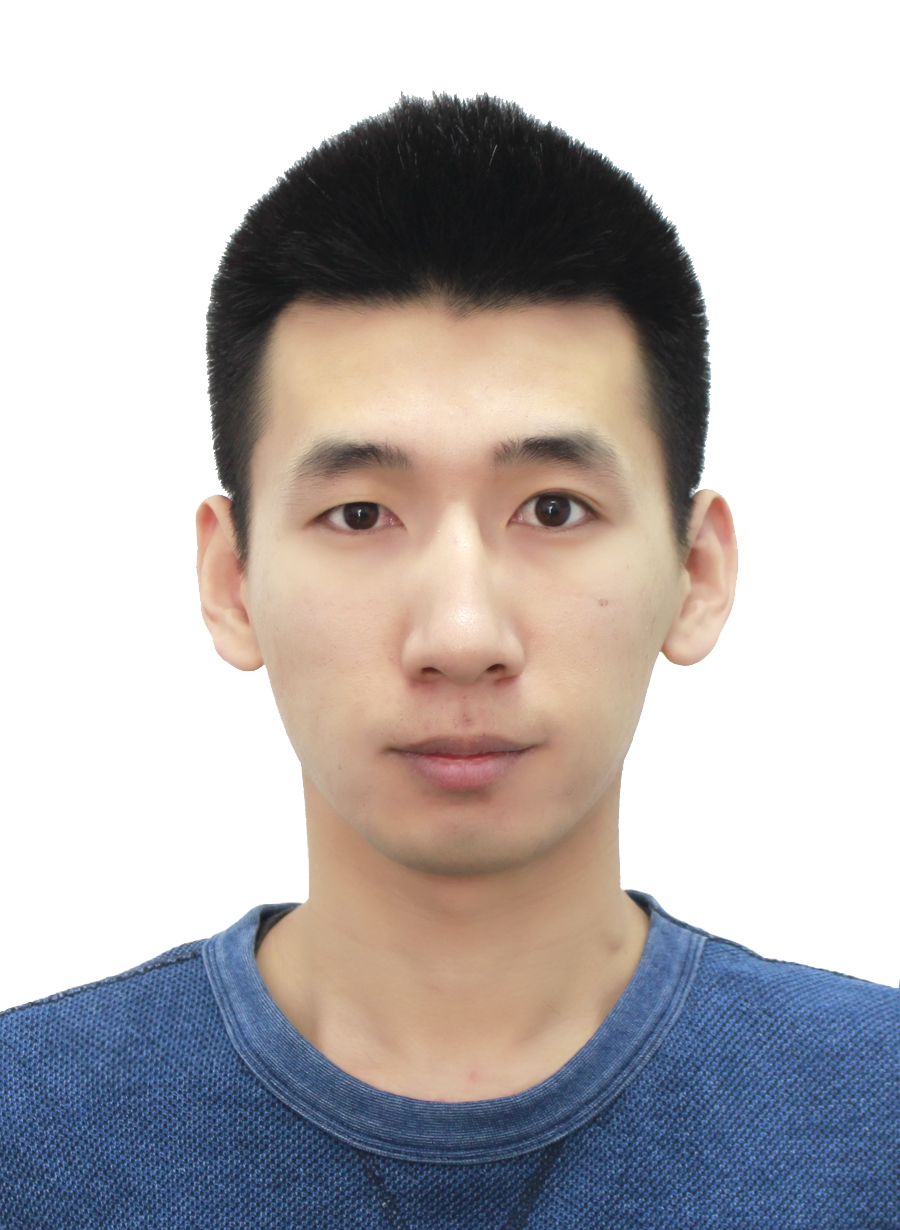
\includegraphics[width=1in,height=1.25in,clip,keepaspectratio]{me.png}}]{Hecheng Zhao} received the B.S. degree
in Automation from
the Nanjing University of Posts and Telecommunications,
Nanjing, China, in 2015. He is currently pursuing the M.S. degree in AI and Robotics with Sungkyunkwan University,
Suwon, South Korea.
His research interests include SLAM, machine learning, and computer vision.
\end{IEEEbiography}

\begin{IEEEbiography}[{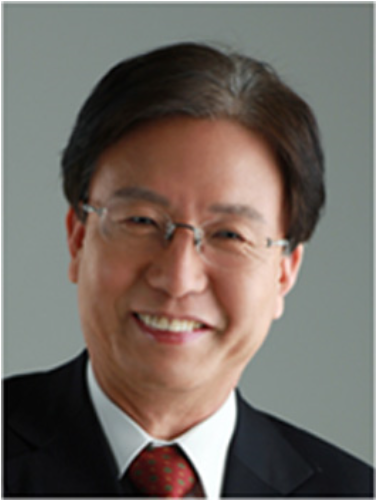
\includegraphics[width=1in,height=1.25in,clip,keepaspectratio]{lee.png}}]{Sukhan Lee}  received the B.S. and M.S. degrees
in electrical engineering from Seoul National
University, South Korea, in 1972 and 1974, respectively, and the Ph.D. degree in electrical engineering from Purdue University, West Lafayette, IN,
USA, in 1982.
From 1983 to 1997, he was with the Departments of Electrical Engineering and of Computer
Science, University of Southern California. From
1990 to 1997, he was with the Jet Propulsion
Laboratory, California Institute of Technology, as a Senior Member of the
Technical Staff. From 1998 to 2003, he was the Executive Vice President,
and also the Chief Research Officer with the Samsung Advanced Institute
of Technology. He has been working as a Professor of information and
communication engineering and WCU Professor of interaction science with
Sungkyunkwan University, since 2003. He was designated the Dean of the
Graduate School of Sungkyunkwan University, in 2011.He is also serving
as the Director of the Intelligent Systems Research Institute. His research
interests are in the areas of cognitive robotics, intelligent systems, and
micro/nano electro-mechanical systems.
Dr. Lee is currently a Fellow of the Korean National Academy of Science
and Technology.
\end{IEEEbiography}

\EOD

\end{document}
